
\section{Quantum Approximate Optimisation Algorithm (QAOA)} \label{sec:qaoa}
    Combinatorial optimisation problems can be formulated by specifying $n$ bits and $m$ clauses, where each clause is a constraint on a subset of the bits. These clauses are satisfied for certain assignments and unsatisfied for others. The objective function $C:\{0,1\}^n\to\mathbb{Z}$ defined on $n$ bit strings, is the number of satisfied clauses given by 
    \begin{equation}
        C(x) = \sum^m_{\mu=1}C_\mu(x),
    \end{equation}
    where $x=x_1x_2\dots x_n$ is the bit string and $C_\mu(x)=1 $ if it satisfies the clause $C_\mu$ or 0 otherwise. For approximation optimisation algorithms, there is a guaranteed ratio on how close the approximate solution is to the optimum of the problem, that is, a bitstring $x'\in\{0,1\}^n$ is guaranteed to be produced with a high probability satisfying
    \begin{equation}
        C_{max}\geq C(x')\geq rC_{max},
    \end{equation}
    where $C_{max} = \underset{x}{\max}\,C(x)$.

    QAOA attempts to find an approximate solution to combinatorial optimisation problems using a variational quantum approach. Variational quantum circuits train an ansatz, a quantum operation that depend on a set of parameters $\pmb{\theta}$. The ansatz is trained using a hybrid quantum-classical loop to solve the optimisation problem
    \begin{equation}
        \pmb{\theta^*} = \underset{\pmb{\theta}}{\arg\min} \, C(\pmb{\theta}).
    \end{equation}

    %Variational Quantum Algorithms are often seen as a promising method of achieving quantum advantage on near term devices. In a lot of cases they do not require the execution of deep quantum circuits and systematic errors can partly be mitigated by outsourcing the optimization procedure to a classical optimizer. Nevertheless, VQAs also face a number of challenges, in particular the questions of whether they are efficiently trainable and produce solutions that are in fact superior to those obtained by classical algorithms. Despite these challenges, VQAs have been proposed for a variety of problem settings, amongst others the following.
    
    There are three components in a QAOA mapping on a problem instance on $n$ binary variables $x\in\{0,1\}^n$ which consists of:
    \begin{enumerate}
        \item An \emph{initial quantum state}, which is taken to be the uniform superposition of all computational basis states of $x$ given by 
        \begin{equation}
            |s\rangle =|+\rangle ^{\otimes n} = \frac{1}{\sqrt{2n}}\sum^{2n-1}_{n=0}|x\rangle,
        \end{equation}
        where $|+\rangle = (|0\rangle+|1\rangle)/\sqrt{2}$.
        \item The \emph{problem Hamiltonian} (or \emph{cost Hamiltonian} as this is the ``cost function''), given by 
        \begin{equation}
            U(C,\gamma) = e^{-i\gamma C} = \prod^m_{\mu=1}e^{-i\gamma C_\mu}.
        \end{equation}
        \item The \emph{mixing Hamiltonian}, given by 
        \begin{equation}
            U(B,\beta) = e^{-i\beta B} = \prod^n_{\nu=1} e^{-i\beta \sigma^x_\nu}.
        \end{equation}
    \end{enumerate}
    For $p\in \mathbb{N}$, there are $2p$ variational parameters that govern the QAOA circuit. Since $C$ has integer eigenvalues, we take $\pmb{\gamma} =(\gamma_1,\dots,\gamma_p)$ where $\gamma_i\in[0,2\pi]$, and $\pmb{\beta} = (\beta_1,\dots,\beta_p)$ where $\beta_i\in[0,\pi]$. The variational state obtained after depth $p$ is given by 
    \begin{equation}
        |\psi_p(\pmb{\gamma},\pmb{\beta})\rangle = U(B,\beta_p)U(C,\gamma_p)\dots U(B,\beta_1)U(C,\gamma_1)|s\rangle,
    \end{equation}
    where the variational parameters are found using a classical optimiser. The optimal parameters that maximise the expectation value is given by $(\pmb{\gamma^*},\pmb{\beta^*})$, where
    \begin{equation}
        (\pmb{\gamma^*},\pmb{\beta^*}) = \underset{\pmb{\gamma},\pmb{\beta}}{\arg\max}\, \langle C\rangle,
    \end{equation}
    and $\langle C\rangle$ is the expectation value given by 
    \begin{equation}
        \langle C \rangle = \langle \psi_p (\pmb{\gamma},\pmb{\beta})| C |\psi_p(\pmb{\gamma},\pmb{\beta})\rangle .
    \end{equation}

    \subsection{Applying QAOA to Number Partitioning}

    Since NPP and max-cut are NP-complete, we can formulate the NPP as an instance of max-cut so that we can apply QAOA to find optimal solutions. Let $S=\{n_1,\dots,n_N\}$ be an NPP. Consider the complete weighted $N$-vertex graph $G=(V,E)$ where each $i\in V$ takes on the value $n_i$ and each edge has weight $w_{ij} = n_in_j$. Then, the optimal weighted max-cut of the graph partitions the vertices into the optimal solution to the original NPP. Figure \ref{fig:number_maxcut} gives an example of an NPP solved using max-cut. We can represent the cost Hamiltonian of the NPP in terms of the cost Hamiltonian of max-cut as
    \begin{align} \label{eq:cost}
        H_{NPP} &= \lr(){\sum^N_{i=1}n_i\sigma_i^z}^2 \nonumber \\ 
        &= 2\sum_{i<j}n_in_j\sigma_i^z\sigma_j^z + \sum^N_{i=1}n_i^2  \nonumber\\ 
        &= -4H_{MC} + 2\sum_{i<j}n_in_j + \sum^N_{i=1}n_i^2  \nonumber \\ 
        &= -4H_{MC} + \lr(){\sum^N_{i=1}n_i}^2.
    \end{align}

    \begin{figure}
        \begin{center}
        \vspace{1cm}
            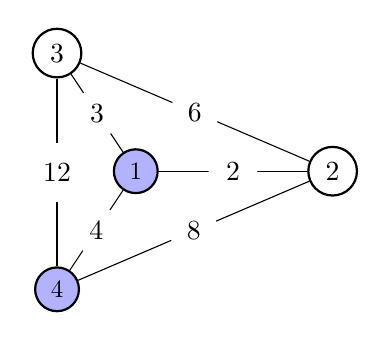
\begin{tikzpicture}
                \begin{scope}[every node/.style={circle,thick,draw},
                    blue/.style={scale=.9, auto=center, circle, draw=black, fill=blue!30, thick, minimum size=6mm}]
                    \node[blue] (1) at (-1.5,0) {1};
                    \node (2) at (1,0) {2};
                    \node (3) at (-2.5,1.5) {3};                       
                    \node[blue] (4) at (-2.5,-1.5) {4};
                \end{scope}
                \begin{scope}[>={[black]},
                    every node/.style={fill=white,circle}]
                    \draw (1) edge node{2}  (2);
                    \draw (4) edge node{8}  (2);
                    \draw (2) edge node{6}  (3);
                    \draw (1) edge node{3}  (3);
                    \draw (1) edge node{4}  (4);
                    \draw (3) edge node{12} (4);
                \end{scope}
                
            \end{tikzpicture}
        \end{center}
        \vspace{0.4cm}
        \caption{The set $S=\{1,2,3,4\}$ can be partitioned into subsets $S_1=\{1,4\}$ and $S_2=\{2,3\}$. When the partition problem is transformed into a complete graph, this partition corresponds to the maximum cut of $12+3+2+8= 25$.}
        \label{fig:number_maxcut}
    \end{figure}

    For depth $p=1$, we provide an analytical form to finding the expectation value of the cost function of QAOA on the max-cut formulation of an NPP in terms of $\beta$ and $\gamma$. We denote this cost as QAOA$_1$.
    \begin{widetext}
        \begin{theorem} \label{thm:qaoa}
            Consider the QAOA$_1$ state $|\gamma,\beta\rangle$ of an NPP transformed into a max-cut problem for a graph $G=(V,E)$. Then the expectation value of the cost $\langle C_{uv}\rangle$ for each edge $\{u,v\}\in E$ is given by
            \begin{align*}
                \left\langle C_{u v}\right\rangle & =\frac{w_{u v}}{2}+\frac{w_{u v}}{4}\left[\sin 4 \beta \sin \gamma_{u v}^{\prime}\left(\prod_{w \in F} \cos \gamma_{w v}^{\prime}+\prod_{w \in F} \cos \gamma_{u w}^{\prime}\right)\right. \\ 
                & \left.+\sin ^2 2 \beta \left(\prod_{w \in F} \cos \left(\gamma_{u w}^{\prime}+\gamma_{v w}^{\prime}\right)-\prod_{w \in F} \cos \left(\gamma_{u w}'-\gamma_{v w}^{\prime}\right)\right)\right],
            \end{align*}
            where $F = V\setminus\{u,v\}$ and $\gamma'_{uv} = -4w_{uv}\gamma_{uv}$.
        \end{theorem}
    \end{widetext}
        \begin{proof}
            We simplify Equation 13 of \cite{vijendran2023expressive} for a complete graph using our formulation of an NPP as a max-cut problem. For complete graphs, we have that $e=d=F$, where $e=\mathcal{N}(v)\setminus\{u\}$, $d=\mathcal{N}(u)\setminus\{v\}$, and $F=\mathcal{N}(u)\cap\mathcal{N}(v)$. By definition, those product terms become 1, returning the simplified result after renaming.
        \end{proof}
        Since Theorem \ref{thm:qaoa} finds the expectation value for each edge, we simply sum the expectation values over all edges of a graph to find the overall expectation value for QAOA$_1$. For complete, $n$-vertex graphs like the instances that we are considering, when we transform an NPP into a max-cut problem, the number of edges is given by $\binom{n}{2}$, yielding $\mathcal{O}(n^2)$ operations. We also see that there are $n-2$ nodes to consider in the set $F$ for a given edge, which means that the product terms are calculated in $\mathcal{O}(n)$ time. Therefore, calculating the expectation value for a graph at depth $p=1$ can be found in $\mathcal{O}(n^3)$ time. However, we note that to find a bitstring that encodes an approximate solution to the graph requires the measurement of a quantum circuit that represents the problem (see {\color{red} assignment document and notebook} for more details).

\subsection{Multi-Angle QAOA (MAQAOA)}
    
    The Multi-Angle QAOA (MAQAOA) varies from QAOA by introducing angle parameters for each summand of the cost and mixing operators as opposed to having a single angle parameter for the cost operator and a second angle for the mixing operator. The angles are chosen to provide more flexibility in optimising the circuit's parameters and improving the algorithm's performance as it is able to explore and determine the feasibility of different solutions more efficiently \cite{herrman2022multi}. 

    For MAQAOA, the problem and mixing Hamiltonians are defined respectively as 
    \begin{align}
        U(C,\pmb{\gamma}) &= e^{-i\sum_\mu\gamma_\mu C_\mu}= \prod^m_{\mu=1}e^{-i\gamma_\mu C_\mu}, \text{ and} \\
        U(B,\pmb{\beta}) &= e^{-i\sum_\nu\beta_\nu B_\nu} = \prod^n_{\nu=1}e^{-i\beta_\nu \sigma^x_\nu},
    \end{align}
    where $\pmb{\gamma} = (\gamma_1,\dots,\gamma_m)$ and $\pmb{\beta} = (\beta_1,\dots,\beta_n)$. For depth $p=1$, MAQAOA would then generate a state of the form 
    \begin{align}
        |\pmb{\gamma},\pmb{\beta}\rangle &= U(B,\pmb{\beta})U(C,\pmb{\gamma})|s\rangle \nonumber \\
        &= \prod^m_{\mu=1}e^{-i\gamma_\mu C_\mu}\prod^n_{\nu=1}e^{-i\beta_\nu \sigma^x_\nu}|s\rangle.
    \end{align}
    \citet{herrman2022multi} proved that MAQAOA guarantees an exact solution as $p\to \infty$. We again present the analytical formula for the expectation value of the cost function of MAQAOA on max-cut formulation of an NPP. We denote this cost as MAQAOA$_1$.   

    \begin{widetext}
    \begin{theorem} \label{thm:maqaoa}
        Consider the MAQAOA$_1$ state $|\mathbf{\gamma,\beta}\rangle$ for an NPP transformed into a max-cut problem for a graph $G=(V,E)$. Then, the expectation value of the cost function $\langle C_{uv}\rangle$ on an edge $\{u,v\}\in E$ is given by
        \begin{align*}
            \langle C_{u v}\rangle & =\frac{w_{u v}}{2}+\frac{w_{u v}}{2}\left[\cos 2 \beta_u \sin 2 \beta_v \sin \gamma_{u v}^{\prime} \prod_{w \in F} \cos \gamma_{w v}^{\prime}+\sin 2 \beta_u \cos 2 \beta_v \sin \gamma_{u v}^{\prime} \prod_{w \in F} \cos \gamma_{u w}^{\prime}\right. \\ 
            & \left.+\frac{1}{2} \sin 2 \beta_u \sin 2 \beta_v \left(\prod_{f \in F} \cos \left(\gamma_{u f}^{\prime}+\gamma_{v f}^{\prime}\right)-\prod_{f \in F} \cos \left(\gamma_{u f}-\gamma_{v f}^{\prime}\right)\right)\right],
        \end{align*}
        where $F = V\setminus\{u,v\}$ and $\gamma'_{uv} = -4w_{uv}\gamma_{uv}$.
    \end{theorem}
    \end{widetext}
    \begin{proof}
        Following the same process as the proof to Theorem \ref{thm:qaoa} yields the result.
    \end{proof}


    Similar to QAOA, finding the total expectation value for a complete graph encoding an NPP has time complexity $\mathcal{O}(n^3)$. However, compared to QAOA which has only two variational parameters, MAQAOA requires $|V|+|E|=\mathcal{O}(n)+\mathcal{O}(n^2)$ variational parameters needing to be optimised.

\subsection{eXpressive QAOA (XQAOA)}

    eXpressive QAOA (XQAOA) is a generalisation of MAQAOA, providing the algorithm with more flexibility to traverse even more possible solutions \cite{vijendran2023expressive}. It defines a new $\pmb{\alpha}$-dependent operator $U(A,\pmb{\alpha})$ given by
    \begin{equation}
        U(A,\pmb{\alpha}) = e^{-i\sum_j\alpha_jA_j} = \prod^n_{j=1}e^{-i\alpha_j\sigma^y_j},
    \end{equation}
    where $\alpha_j\in[0,\pi]$. We then let the mixing Hamiltonian be the product of $U(B,\pmb{\beta})$ and $U(A,\pmb{\alpha})$. For depth $p=1$, XQAOA would then generate a state of the form 
    \begin{align}
        |\pmb{\gamma},\pmb{\beta},\pmb{\alpha}\rangle &= U(A,\pmb{\alpha})U(B,\pmb{\beta})U(C,\pmb{\gamma})|s\rangle \nonumber \\
        &= \prod^n_{\nu=1}e^{-i\alpha_\nu \sigma^y_\nu}e^{-i\beta_j\sigma^x_j}\prod^m_{\mu=1}e^{-i\gamma_\mu C_\mu}|s\rangle,
    \end{align}
    where $\pmb{\alpha}=(\alpha_1,\dots,\alpha_n)$, $\pmb{\beta} = (\beta_1,\dots,\beta_n)$, and $\pmb{\gamma} = (\gamma_1,\dots,\gamma_m)$.
    %\begin{theorem}

        

        %Consider the $XQAOA$ state $|\mathbf{\gamma,\beta,\alpha}\rangle$ for depth $p=1$. Let $G=(V,E)$ be a weighted graph with each edge $\{u,v\}\in E$ weighted by $w_{uv}$. Then, the expectation value of the cost function $\langle C_{uv}\rangle$ on an edge $\{u,v\}\in E$ is
        
        %\begin{align}
        %    \begin{split}
        %    \langle C_{uv}\rangle &= \frac{w_{uv}}{2}+\frac{w_{uv}}{2}\Bigg[\cos2\alpha_u\cos2\alpha_v\sin\gamma'_{uv}\lr(){\cos2\beta_u\sin2\beta_v\prod_{w\in e}\cos\gamma'_{wv}+\sin2\beta_u\cos2\beta_v\prod_{w\in d}\cos\gamma'_{uv}}   \\
        %     &-\frac{1}{2}\sin2\alpha_u\sin2\alpha_v\prod_{\substack{w\in e \\ w\notin F}}\cos\gamma'_{wv}\prod_{\substack{w\in d \\ w\notin F}}\cos\gamma'_{uw}\lr(){\prod_{f\in F} \cos(\gamma'_{uf}+\gamma'_{vf})+\prod_{f\in F}\cos(\gamma_{uf}-\gamma'_{vf})} \\
        %    & +\frac{1}{2}\cos2\alpha_u\sin2\beta_u\cos2\alpha_v\sin2\beta_v\prod_{\substack{w\in e \\ w\notin F}}\cos\gamma'_{wv}\prod_{\substack{w\in d \\ w\notin F}}\cos\gamma'_{uw}\Bigg(\prod_{f\in F}\cos(\gamma'_{uf}+\gamma'_vf)-\prod_{f\in F}\cos(\gamma_{uf}-\gamma'_{vf})\Bigg)\Bigg],
        %    \end{split}
        %\end{align}
        %where $\gamma'_{jk} = \gamma_{jk}w_{jk}$.
   % \end{theorem}

    \begin{widetext}
    \begin{theorem} \label{thm:xqaoa}
        Consider the $XQAOA$ state $|\pmb{\gamma},\pmb{\beta},\pmb{\alpha}\rangle$ for an NPP transformed into a max-cut problem for a graph $G=(V,E)$. Then, the expectation value of the cost function $\langle C_{uv}\rangle$ on an edge $\{u,v\}\in E$ for depth $p=1$ is given by
        \begin{align*}
            \begin{split}
                %\langle C_{uv}\rangle_{NP} &= -4\langle C_{uv}\rangle + 
            \langle C_{uv}\rangle &= \frac{w_{uv}}{2}+\frac{w_{uv}}{2}\Bigg[\cos2\alpha_u\cos2\alpha_v\sin\gamma'_{uv}\lr(){\cos2\beta_u\sin2\beta_v\prod_{w\in F}\cos\gamma'_{wv}+\sin2\beta_u\cos2\beta_v\prod_{w\in F}\cos\gamma'_{uv}}   \\
             &-\frac{1}{2}\sin2\alpha_u\sin2\alpha_v\lr(){\prod_{w\in F} \cos(\gamma'_{uf}+\gamma'_{vf})+\prod_{w\in F}\cos(\gamma'_{uf}-\gamma'_{vf})} \\
             & +\frac{1}{2}\cos2\alpha_u\sin2\beta_u\cos2\alpha_v\sin2\beta_v\Bigg(\prod_{w\in F}\cos(\gamma'_{uf}+\gamma'_vf)-\prod_{w\in F}\cos(\gamma'_{uf}-\gamma'_{vf})\Bigg)\Bigg],
            \end{split}
        \end{align*}
        where $F=V \setminus \{u,v\}$ and $\gamma'_{uv} = -4w_{uv}\gamma_{uv}$.
    \end{theorem}
    \end{widetext}
    \begin{proof}
        Following the same process as the proof to Theorem \ref{thm:qaoa} yields the result.
    \end{proof}

    Several variants of XQAOA were proposed by \citet{vijendran2023expressive}. For our simulations with XQAOA, we apply the X=Y mixer variant XQAOA$^{\text{X=Y}}$ where we set $\alpha=\beta$ as it was found to have the best approximation ratio of max-cut for $D$-regular graphs of degree 3-10 with 128 and 256 vertices. We denote this cost as XQAOA$_1^\text{X=Y}$.
